\documentclass[a4paper,10pt]{article}
\usepackage[utf8]{inputenc}
\usepackage{amsbsy}
\usepackage{fixltx2e}
\usepackage{amsfonts}
\usepackage{natbib}
\usepackage{graphicx}
\usepackage{mathtools}
\usepackage{xcolor}
\usepackage{color} 
\usepackage{hyperref}
\usepackage{tcolorbox}
\usepackage{mathrsfs}
\usepackage{amssymb}
\usepackage{appendix}
\usepackage{amssymb}
\usepackage{amsthm}
\usepackage{fancyhdr}
\usepackage[T1]{fontenc}
\usepackage[utf8]{inputenc}
\usepackage{lmodern}
\usepackage{minted}
\usepackage{algorithm}
\usepackage{algpseudocode}
\def\code#1{\texttt{#1}}
\usepackage{amsthm}
\newtheorem{definition}{Definition}
\usepackage[letterpaper,top=2cm,bottom=2cm,left=3cm,right=3cm,marginparwidth=1.75cm]{geometry}
\usepackage[colorinlistoftodos,prependcaption]{todonotes}
\hypersetup{
    colorlinks=true,
    linkcolor=blue,
    filecolor=magenta,      
    urlcolor=cyan,
    pdftitle={Overleaf Example},
    pdfpagemode=FullScreen,
    }
\usepackage{minted}




\begin{document}

%TITLE PAGE
\begin{titlepage}
   \begin{center}
       \vspace*{1cm}

       \textbf{Quadratic Assignment Problem}

       \vspace{0.5cm}
        A study on the performance of various heuristic methods
            
       \vspace{1.5cm}

        
       \textbf{Author(s):} Sean Conlon, Qiaoyang Xu, Hongqing Wei  \\

       \vfill
            
       Submitted as group project for \texttt{MAST90098} Approximation Algorithms \& Heuristics
            
       \vspace{0.8cm}
     
       
\includegraphics[width=0.3\textwidth]{images/uomlogo.png}
            
       School of Mathematics \& Statistics \\
       The University of Melbourne\\
            
   \end{center}
\end{titlepage}

%%TABLE OF CONTENTS%%
\tableofcontents
\thispagestyle{empty}
\clearpage
\setcounter{page}{1}



\newpage
\section{Introduction}
Within this project we study the Quadratic Assignment Problem (QAP), which is a fundamental problem of  optimisation and operations research. 

\subsection{Problem Motivation}
QAP is an important subject of research for its computational difficulty, as well as for it's wide applicability to a number of domains. Within this short paper, we review recent works on suitable approximations to the problem, as well as empirically test these approximations on a suitable instance of the problem.


\label{Definition 1}
\begin{definition}[Quadratic Assignment Problem] Given two sets facilities $F$ and locations $L$ of equal size with weight function $w: F\times F \rightarrow \mathbb{R}$ and distance function $d: L\times L \rightarrow \mathbb{R}$ determine the one-to-one mapping function $f: F \rightarrow L$ such that 
$$cost := \sum_{i,j\in F} w_{i,j}d_{L(i),L(j)}$$
is minimised, where $L(i)$ maps to the location of facility $i$. Representing the weight and distance functions as square matrices $W$ and $D$, the problem is equivalent to determining the permutation matrix minimising 
$$\text{trace}(WXDX^T)$$
\end{definition}
QAP arises in a number of domains within applied operations research, where one considers the optimal layout of facilities such that the distance between said facilities weighted by their reflected flows is minimised. A particularly interesting and well researched application of QAP is to the design of hospital layout \cite{Elshafei}; Hospitals maintain a number of important facilities such as emergency rooms, ongoing care, specialist centers, ect, with nurses, doctors and other medical professionals needing to move quickly between such facilities. An optimal layout for a hospital therefore, would seek to minimise the distance between critical facilities where many medical professionals move between, which is precisely modelled by the objective function of the QAP in \ref{Definition 1}. \\
\\
QAP also provides a general formulation for a number of important discrete optimisation problems. For example, consider the Travelling Salesman Problem (TSP) defined as follows:
\begin{definition}[Travelling Salesman Problem]
Given a list of cities $1,\dots,n$ which we denote as $x_1, \dots, x_j$ with cost $c_{ij}>0$ to traverse from city $i$ to city $j$ determine the lowest tour length corresponding to
$$\text{cost} = \sum_{i=1}^{n}\sum_{j\neq i, j=1}^{n}c_{ij}x_{ij}$$
\end{definition}
Being an \href{https://en.wikipedia.org/wiki/NP-completeness}{NP Complete Problem} \cite{Sahni}, TSP is one of the most well studied and important computational problems in Computer Science. Indeed, TSP can be viewed as a special instance of QAP if one considers the set of facilities to be the cities $\{1,\dots,n\}$ and set $d_{i,j} = c_{i,j}$ along with weights $w_{i,j} = 1$. Other important discrete optimisation problems such as maximal clique, graph partitioning can have also been shown to be formulated as instances of QAP \cite{Loiola07}. \\
\\
Given this power to model a number of practical and theoretically important problems, there is natural motivation from practitioners and the research community in designing effective heuristics for the QAP problem.

\newpage
% QI's TODO! 
\subsection{Literature Review}

\subsubsection*{Computational Complexity }


The QAP (Quadratic Assignment Problem) is a classic real-world optimization problem. Over centuries of research, mathematicians have developed a better understanding of QAP, categorizing its problems and solutions. In this section, we'll introduce key insights from their work.


In\cite{article}, They presented nine QAP formulations, including Koopmans–Beckman QAP, Quadratic 0–1, Mixed Integer Linear Programming (MILP), Permutation, Trace, Semidefinite Programming Relaxation (SDP), Graph, Kronecker Product, and Concave Quadratic formulations.

In 2003, Anstreicher\cite{Anstreicher2003RecentAI}, the author of 'Recent Advances in Solving Quadratic Assignment Problems,' summarized all algorithms for solving QAP. To solve QAP, both lower-bound and exact solution algorithms are necessary.




QAP problems are categorized as NP-hard. While exact algorithms like cutting planes, branch and bound, branch and cut, and dynamic programming can find optimal solutions for small instances, they become highly inefficient for very large instances due to the existence of n! permutations. In such cases, heuristics and metaheuristic algorithms are preferred for faster optimal solutions.


\subsubsection*{A summary of research on Constructive Heuristics}

Constructive heuristics, employed in optimization and combinatorial problems like QAP, involve a step-by-step approach to problem-solving. By employing decision-making processes that involve the selection of components or elements to gradually assemble a solution. These strategies find application in optimization problems, search algorithms, and various decision-making contexts. Notably, Arkin et al. (2001) \cite{ARKIN200113} utilized this approach, this is one of the oldest methods for solving QAP. It begins with an empty set, incrementally builds the solution with more detail, and iterates until an optimal solution is reached or no further progress is possible. This approach differs from Local Search Heuristics, which start from an optimal solution and seek improvements by exploring neighboring solutions.

Some algorithms for Constructive Heuristics: 

Greedy algorithm:
Description: Greedy Set Cover starts with an empty set and iteratively selects the set that covers the most uncovered elements, thus incrementally covering the entire ground set.

Randomized Greedies:  a class of algorithms that combine elements of both greedy algorithms and randomization to find approximate solutions to optimization problems. These algorithms introduce randomness into the selection process, which can lead to different results on different runs. Randomized Greedies are particularly useful when dealing with NP-hard problems where finding an optimal solution is computationally infeasible, and a near-optimal solution is acceptable.

Overall, Constructive heuristics prove their worth in scenarios where the pursuit of an optimal solution is either computationally demanding or unattainable, and where achieving a solution of good quality suffices. Furthermore, they can serve as an initial step for more intricate optimization algorithms or be integrated with other heuristic techniques to enhance the overall quality of the solution.

\subsubsection*{A summary of research on Meta heuristics}
For the 
Metaheuristics are used to address a variety of optimization problems and are divided into two main classes: single-based solutions and population-based solutions. Single-based solutions begin with one candidate solution and iteratively improve it. Population-based solutions work with a group of solutions, initially chosen randomly, and iteratively enhance the population using algorithms like genetic algorithms. Comparing these two classes, population-based solutions are often preferred because they facilitate information sharing among solutions and help avoid local optima. Metaheuristics are influenced by both theoretical and experimental factors and can draw inspiration from natural processes \cite{article}. Additionally, combining two or more Metaheuristics can yield better solutions than using a single Metaheuristic \cite{article}.

Here are descriptions of several well-known metaheuristics:

Genetic Algorithms (GA): GA draws inspiration from natural selection. It involves evolving a population of potential solutions over multiple generations, employing genetic operations like mutation and crossover to simulate the genetic evolution process.

Simulated Annealing: Simulated Annealing takes its cue from the annealing process in metallurgy. It employs temperature-based strategies to systematically explore the solution space, allowing it to move away from local optima and reach more promising areas.

Ant Colony Optimization (ACO): ACO is influenced by the foraging behavior of ants. It utilizes pheromone trails to guide the search for solutions in complex combinatorial spaces, mimicking how ants find optimal paths.

Particle Swarm Optimization (PSO): PSO is inspired by the social behavior of birds or fish. It models particles (representing solutions) that adjust their positions based on their own experiences and the collective wisdom gained from their peers, leading to solution improvement.

Tabu Search: Tabu Search maintains a list of "tabu" moves, which cannot be revisited. This strategy prevents the algorithm from becoming trapped in cycles and ensures it explores the neighborhood of solutions more effectively.

These metaheuristics offer innovative approaches to solving complex optimization problems, each drawing inspiration from different natural or social phenomena.


\newpage
\section{Methods}
Recalling the definition of QAP \ref{Definition 1}, a solution to an instance of the QAP is a permutation of the facilities minimising the sum of weight-distance products. For a QAP instance on $n$ sites and facilities, utilising a brute-force approach scales at a rapidly prohibitive $O(n!)$ time complexity. To circumvent infeasible compute time, we forgo exactly solvable methods in favour of heuristics to develop approximately correct solutions. \\
\\
In the below sections of our paper, we propose and explain a number of different hueristics for the QAP.

\subsection{Constructive Heuristics}
Constructive Heuristics develop approximated solutions by initialising an empty permutation, and then constructing a full assignment of facilities to locations. To implement a constructive heuristic, we must define a strategy for \textit{adding} to the current \textit{solution} under construction. For QAP and a number of other combinatoral optimisation problems such as TSP, this is typically via a greedy selection. 

\subsubsection*{Simple Greedy}
We propose the below algorithm which is perhaps the simplest design for a greedy constructive heuristic. The algorithm works by maintaining a set of assigned facilities which is intially set to be empty, and on every step of the algorithm, assign to position $i$ the facility $j$ such that: 
\begin{enumerate}
    \item $j$ is so far unassigned and
    \item $j$ minimises the cost function defnied in  Definition \ref{Definition 1}.
\end{enumerate}
Described in psuedocode this algorithm can be implemented as follows: 

\begin{algorithm}
\caption{Simple Greedy}\label{alg:cap}
\begin{algorithmic}
\State $s \gets $ Empty Solution
\State $Assigned Facilities \gets \emptyset$
\For {location $i=1,\dots,n$}
    \State $s[i] \gets OptimalFacility(i, AsssignedFacilities)$
    \State $AssignedFacilities \gets AssignedFacilities \cup \{s[i]\}$
\EndFor
\State return $s$
\end{algorithmic}
\end{algorithm}

Our algorithm proposed above has a few main benefits; firstly that is immediately intuitive and unlike other methods, requires no hyper parameter tuning. Additionally, the algorithm is incredibly efficient to compute, with a total run time of $O(n^2)$ when implemented naively. Using more advanced techniques for determining the optimal facilitiy \cite{KHULLER199534} can also be used to bring the computational runtime to be sub-quadratic. Given that $n\leq 256$ for all of our test instances however, we simply compute the optimal facility naively through a linear scan. \\
\\
One shortfall of our simple greedy approach however is the order in which we assign facilities to locations is fixed, starting from location $i=1$ up to $n$. Similar to a greedy knapsack algorithm, this can result in very sub optimal orderings, with facilities that would be more beneficially located to later locations possibly being assigned to earlier facilities. As seen by our results in section 3, this can lead to rather poor approximations. Fortunately however, given we can compute Algorithm 1 rather efficiently, we can remedy this through generating a number of randomised location orders, and then running multiple instance of Algorithm 1. This idea forms the basis of our first randomised greedy algorithm.


\subsubsection*{Randomized Greedy I}
By randomising the order in which we insert the locations in our main foor loop of Algorithm 1, we can generate wildly different approximations of the optimal solution. Our algorithm is a simple extension of Algorithm 1; take some integer $k$ of different insertion orders, run Algorithm1 on each of the insertion orders to result in $k$ different assignments, and then return the assignment that results in the lowest cost. Written in psuedo-code: 

\begin{algorithm}
\caption{Randomised Greedy}\label{alg:cap}
\begin{algorithmic}
\Require number of iterations $k_{max}$
\State $solutions\gets \emptyset$
\For{$k = 1,\dots k_{max}$}
\State $s \gets $ Empty Solution
\State $Assigned Facilities \gets \emptyset$
\For {location $i$ in random permutation of $\{1,\dots,n\}$}
    \State $s[i] \gets OptimalFacility(i, AsssignedFacilities)$
    \State $AssignedFacilities \gets AssignedFacilities \cup \{s[i]\}$
\EndFor
\State $solutions \gets solutions \cup \{s\}$
\EndFor
\State return $\arg \min solutions$
\end{algorithmic}
\end{algorithm}
The runtime of Algorithm 2 is clearly $O(k_{max}n^2)$ and follows from our analysis of Algorithm 1. Given the efficiency in which we can compute the inner loop, we set $k_{max}\gg n$ in our experiments, and were pleased some significantly improved results. \\
\\
There are some shortfalls to Algorithm 2 however, the first is that the approximation quality depends largely on the difference and \textit{quality} of the $k$ random insertion orders that are generated. As even for $k$ in the millions of iterations is dwarfed by the size of the $n!$ total permutations, running different instances on Algorithm 2 on the same QAP can still result in potentially massive gaps in approximation quality. As mentioned above, this results in some sense of \textit{quality} of an insertion order that cannot be checked \textit{a priori}. This places a heavy emphasis on luck for our Randomised Greedy approach. 

\subsubsection*{Randomized Greedy II}
Randomized Greedy is a variation on the classic greedy heuristic. Instead of always making the absolute best choice at each stage, we introduce randomness, selecting from among the top available choices. This allows the algorithm to explore different solutions in the search space, potentially avoiding local optima.

The pseudocode for a general implementation of the Randomized Greedy algorithm for the Quadratic Assignment Problem (QAP) is as follows:

\begin{algorithm}
\caption{Simplified Randomized Greedy for QAP}\label{alg:very_simple_rg_qap}
\begin{algorithmic}
\Require QAP Instance, Parameter $p$ 
\State $s = [-1,-1,-1...] \gets InitialSolution$
\State $U \gets UnassigndFacilities$
\While{$U \neq \emptyset$}
    \State Find a set of promising candidates $C$ for the next step in $s$
    \State Compute a cost for each candidate in $C$
    \State Sort $C$ based on the computed costs
    \State Select a subset of top $p$ fraction from $C$ as $C'$
    \State Randomly choose a candidate from $C'$ and add to solution $S$
    \State Update $U$
\EndWhile
\State return $s$
\end{algorithmic}
\end{algorithm}

In the context of the QAP, this algorithm builds an assignment of facilities to locations. By introducing randomness via the p parameter, the algorithm can produce diverse solutions, which can be particularly useful when paired with other optimization techniques or when searching vast solution spaces. The core procedures include assigning facilities to locations based on a cost metric, maintaining a list of potential best choices, and periodically introducing randomness to explore various assignments.

The heuristic begins with an initial solution. As it progresses, a "candidate list" of possible moves or elements is generated. Each candidate is evaluated based on a predetermined function, ranking them in terms of their potential benefit to the solution.

But rather than consistently selecting the top candidate, the algorithm introduces an element of unpredictability. From the top-ranked candidates, a subset is identified. A candidate is then randomly picked from this subset for incorporation into the growing solution. As one candidate merges with the solution, the list updates, removing the selected candidate and making room for potential new ones.

This cycle of evaluation, random selection, and list updating continues until the algorithm meets a termination condition. This could be the exhaustion of the candidate list or the achievement of a specific solution quality or iteration count

\newpage
\subsection{Local Search Heuristics}
Heuristics based on local search schema are an intuitive method, based on strategically exploring local regions of the search space. There is a blurred distinction between Metahueristic and Local Search heuristics; and we note that the below methods described may be characterised as metahueristics to some readers. 

\subsubsection*{Simulated Annealing}
Simulated Annealing (SA) is a local search technique, enhanced by a randomisation step that allows the algorithm to escape local optima to develop possibly better solutions. SA has been widely applied to a number of domains and computational problems \cite{SAReview}. For it's wide success and relative ease of implementation, we first implemented SA to act as a benchmark for other local search methods and metaheuristics following the psuedocode described below 

\begin{algorithm}
\caption{Simulated Annealing}\label{alg:cap}
\begin{algorithmic}
\Require maximum number of iterations $k_{max}$, initial temperature $T_0$
\State $s \gets GenerateInitialSolution()$
\While{ convergance criterion not met}
\For {$k=1,\dots,k_{max}$}
    \State $T\gets T_0$
    \State $s^{\prime} \gets neighbor(s) $
    \State \textbf{If} \textit{cost$(s^\prime)$ < cost$(s)$}: then $s\gets s^\prime$
    \State \textbf{Else If}  $\exp(cost(s) - cost(s^\prime))/(k-T)\geq random(0,1)$: $s\gets s^\prime$
\EndFor
    \State Reduce $T$
\EndWhile
\State return $s$
\end{algorithmic}
\end{algorithm}

As one can see from the psuedo code, SA is a generally ready \textit{out of the box} algorithm for producing approximate results for a number of combinatorial problems. When applying SA as specified above, one needs only to describe how to generate a neighbor, as well as generating an initialy solution. \\
\\
For these reasons, we used the following straightforward approaches to defining these methods, and then used SA as a benchmark for fancier metaheuristics and local search methods. Firstly, to generate a neighbor of a given permutation $s$, we use the following procedure

\begin{algorithm}
\begin{algorithmic}
    \Procedure{Neighbor}{$s$}
        \State $p\gets random(0,1)$
        \State \textbf{If} $p<0.1$ return a random shuffle of $s$
        \State \textbf{Else} swap two indices and return $s$ 
    \EndProcedure
\end{algorithmic}
\end{algorithm}

The procedure typically produces a member from the 2-Opt neighborhood of $s$, though with relatively small probability shuffles the solution entirely to encourage exploration of a radically different search space. FInally, to generate an initial solution we simply return a random permuation of $\{1,\dots,n\}$. Given our implementation of the neighbor procedure, and the overall algorithm encourages searching the solution space, we find that using an constructive heuristic in place of a random permutation led to no better results. 

\subsubsection*{Iterated Local Search}
Iterated Local Search (ILS) is a powerful method for solving discrete optimisation problems, based on iteratively exploiting solutions in local search regions, then perturbing the current solution to explore a different region. Psuedocode for a general implementation of ILS is provided below

\begin{algorithm}
\caption{Iterated Local Search}\label{alg:cap}
\begin{algorithmic}
\Require QAP Instance, Termination Condition
\State $s_0 \gets GenerateInitialSolution()$
\State $s \gets LocalSearch(s_0)$
\While{Termination Condition not met}
    \State $s^\prime \gets Perturbation(s)$
    \State $s^{\prime\prime} \gets LocalSearch(s^\prime)$
    \State $s \gets AcceptanceCireterion(s,s^{\prime\prime})$
\EndWhile
\end{algorithmic}
\end{algorithm}
Writing a sufficient algorithm to conduct this transition to different regions of the search space, also known as \textit{perturbation} is a non-trivial task, and requires different consideration for different optimisation problems. Moreover, there is a great deal of flexibility in how we approach other subprocedures, such as the generation of an initial feasible solution, and the local search itself. \\
\\
We leverage prior research on implementing ILS for QAP \cite{stuzle} to guide how we implement the four main procedures.  As noted in the literature \cite{Loiola07, stuzle} as well as in our own results in section 3 and 4 of this paper, QAP does not exhibit reliable constructive heuristics. For this reason, and to save compute time, we generate our initial solution as a simple random permutation

\begin{algorithm}
\begin{algorithmic}
    \Procedure{GenearteIitialSolution}{$n$}
        \State return random permutation of $\{1,\dots,n\}$
    \EndProcedure
\end{algorithmic}
\end{algorithm}
Similarly, we implement the acceptance criterion exactly as specified in \cite{stuzle}, which simply accepts any better proposed solution. 
\begin{algorithm}
\begin{algorithmic}
    \Procedure{AcceptanceCriterion}{$s, s^\prime$}
        \State return argmin $\{\text{cost}(s), \text{cost}(s^\prime)\}$
    \EndProcedure
\end{algorithmic}
\end{algorithm}

The aspect of the model which required most consideration is the perturbation and local search steps. To complete the local search procedure, we use a simple 2-Opt neighborhood of the current solution. Prior research \cite{stuzle} uses a slightly modified technique of \textit{don't look bits}, to reduce the $O(n^3)$ computation of the local search, though we found this needlessly complicated to implement.. \\
\\
Our perturbation procedure exchanges $k$ randomly chosen sites within our permutation; effectively resulting in $k$ being an additional hyper-parameter to our algorithm. Borrowing the results of \cite{stuzle}, it is generally accepted that the optimal choice of $k$ is `\textit{rather dependent on the QAP instance under consideration}', so to make our heuristic more robust, we adapt $k$ over the life of the algorithm.  To adapt $k$, we set $k_{min} = 4$ for all instances. If after a round of local search, no better solution is found, we increment $k \leftarrow k+1$, so as to create a larger perturbation, and more likely to escape local minima. These increment steps can occur all the way up to $k_{max} = n$ for a given input instance. 
 
\begin{algorithm}
\begin{algorithmic}
    \Procedure{LocalSearch}{$s_0$}
        \State return argmin of 2-Opt neighborhood of $s_0$ with respect to cost function
    \EndProcedure
\end{algorithmic}
\end{algorithm}

\begin{algorithm}
\begin{algorithmic}
    \Procedure{Pertubation}{$s, k$}
        \State swap $k$ indices of $s$ at random
    \EndProcedure
\end{algorithmic}
\end{algorithm}







\newpage
\subsection{Metaheuristics}


\subsubsection*{Genetic Algorithm}

Genetic Algorithms (GA) are a class of biology-inspired metaheuristics that work through repeatedly modifying a `population' of solutions. Inspired by natural selection, GA's follow biologically inspired operations of mutating, selecting and crossover of \textit{fit} or \textit{strong} candidate solutions within the population to generate new, hopefully better solutions.\\
\\
Though prior literature has stated that genetic algorithms \textit{have proven to be most effective on non-convex optimisation problems with relatively easy access to the quality of a given feasible solution - which the QAP is not} \cite{TATE199573} - for the sake of completeness as well as out of academic curiosity, we implemented such a heuristic. \\
\\
There are a plethora of well-studied methods to architect a GA, though all roughly follow the following pseudo code: 
\begin{algorithm}
\caption{Genetic Algorithm}\label{alg:cap}
\begin{algorithmic}
\Require QAP Instance, Termination Condition, PopulationSize
\State $P \gets GenerateInitialPopulation(PopulationSize)$
\While{Termination Condition not met}
    \State $p1, p2 \gets SelectParents(P)$
    \State $c \gets Crossover(p_1, p_2)$ \Comment{generate a child from $p_1, p_2$}
    \State $P\gets P\cup\{c\}$
    \State $P \gets mutate(P)$
    \State $P \gets cull(P)$ \Comment{remove unfit members from population}
\EndWhile
\end{algorithmic}
\end{algorithm}
Similar to our implementation of Iterated Local Search - we set our termination to the first to occur between a  number of iterations, or a CPU time of 60 seconds. Beyond that, the genetic algorithm described above provides a great deal of flexibility in how, and how frequently we select, generate crossover and mutate our initial population. We now describe how we implement each of these procedures in our final GA. \\
\\
We first describe how we generate the initial population. Whilst prior research has stated that \textit{GA's are sensitive to the quality of their initial populations} \cite{TATE199573}, other research\footnote{Whilst we cite past research, the paper appears unpublished as it appears to be the part of a M.Sc research project, but accessible through the following \href{https://www.siam.org/Portals/0/Documents/S140619PDF.pdf?ver=2021-08-29-110233-343}{link}. We also found similar results with our relatively simple testing that constructive approaches to generate a \textit{fitter} initial population resulted in no significant changes to the quality of our final solution.} has found that quality of initial populations do not appear to drive statistically significant changes to the quality of the final solution \cite{GAPopulation}. Given these findings, in our final algorithm we simply generate an initial population of 100 random permutations. \\
\\
The \textit{Crossover} method is used to generate a new permutation for given parent permutations from the existing population $p_1, p_2$. Whilst it is not immediately obvious on how to define a valid Crossover function, we borrow inspiration from combinatorial problems involving permutations such as TSP, as well as prior research \cite{1994Improved, GAPopulation}. This led us to considering a simple \href{https://en.wikipedia.org/wiki/Crossover_(genetic_algorithm)}{partially mapped crossover method} in which we leveraged existing implementations online. Additionally, to select the parental permutations for input, we simply choose two members of the population at random. \\
\\
Finally, to perform the remaining methods of \textit{mutate} and \textit{cull}, we simply swap the assignment of $k$ indices at random, and keep only the fittest members of the population in accordance with the \textit{PopulationSize} input. Whilst both techniques are relatively vanilla, they are also straight forward and easy to implement. \\
\\
Whilst we have described and implemented a reasonable GA, we have removed the heuristic from our results detailed in section 3 of this report. The rationale being that we found the convergence results of the algorithm to be poor within the 60 second compute time frame, and our experimental environment a poor measurement of the effectiveness of the algorithm. Moreover we used Simmulated Annealing as a baseline for performance for considering more advanced methods, which our genetic algorithms consistenly failed to outperform. Prior research has identified issues in the convergance of such methods \cite{HE199923}. 
Whilst this exclusion is disappointing, we have included potential methods to improve the method in section 4 of this paper.  


\subsubsection*{Tabu Search}

Having delved into the intricacies of Genetic Algorithms, an evolution-inspired optimization technique, our discussion now pivots to another potent metaheuristic—Tabu Search. Renowned for its innovative utilization of memory structures, Tabu Search stands in contrast to the population-based paradigm of Genetic Algorithms. Specifically, while it emphasizes local exploration, it integrates a memory mechanism to deter repetitive cycles and effectively navigate away from local optima. In the following sections, we shall dissect the mechanisms and advantages of this sophisticated optimization approach.\\
\\
Tabu Search (TS) is an advanced metaheuristic optimization algorithm introduced by Fred Glover in the 1980s \cite{GLOVER1986533}. It is specifically designed to solve combinatorial optimization problems. The hallmark of Tabu Search is its use of adaptive memory, represented primarily through its \textit{tabu list}, to guide the search and aid in escaping from local optima. Here is the pseudo code: 
\begin{algorithm}
\caption{Tabu Search}\label{alg:cap}
\begin{algorithmic}
\Require QAP Instance, Termination Condition, Aspiration Criteria
\State $T \gets TabuList()$
\State $s \gets GenerateInitialSolution$
\State $s_{\text{best}} \gets s$  % Assuming the initial solution is the best-known solution initially
\While{Termination Condition not met}
    \State Find the best move in the neighborhood of s that is not in TabuList or satisfies aspiration criteria
    \State Apply the found best move to s to get a new solution
    \State Update TabuList
    \If{the new solution is better than $s_{\text{best}}$}
        \State $s_{\text{best}} = s$
    \EndIf
\EndWhile
\State Return $s_{\text{best}}$
\end{algorithmic}
\end{algorithm}

TS is a versatile and widely-used metaheuristic designed for solving combinatorial optimization problems. Its main strength lies in its use of memory, specifically the tabu list, to escape local optima and guide the search towards global optima. Below, we'll break down the typical components of a Tabu Search, detailing each procedure.\\
\\
The \textbf{Initialization} phase of the algorithm is crucial. Initially, a solution is either randomly generated or conceived based on a rudimentary heuristic. This initial solution serves as the starting point for the forthcoming search. In our code, we will use the greedy algorithm, as discussed in the previous part, to generate our initial solution.

\begin{algorithm}[H]
\begin{algorithmic}
    \Procedure{GreedyAlgorithm}{$F, D$}
        \State use greedy constructive heuristic to formulate an initial solution s
        \State return s
    \EndProcedure
\end{algorithmic}
\end{algorithm}

In parrallel, the tabu list is initiated. Characteristically, this list archives the last \(n\) moves or solutions that have been explored\cite{GLOVER1999}. The dimension of this list significantly influences the algorithm's behavior. A lengthier list, for instance, acts as a deterrent, preventing the algorithm from cyclically revisiting certain sections of the solution space. However, this also poses a risk, potentially obstructing exploration.\\
\\
As TS progresses into its \textbf{Iterative Search} phase, each solution's neighborhood is thoroughly explored. This exploration often involves elementary moves, like the swapping of two sequence elements\cite{GLOVER1999}. Following the exploration, all neighbors are meticulously evaluated based on a pre-defined objective function, which is a cost function in our code.

\begin{algorithm}[H]
\begin{algorithmic}
    \Procedure{Cost}{$s$}
        \State Compute the cost of solution s by rearranging matrix
        \State return \(cost_s\)
    \EndProcedure
\end{algorithmic}
\end{algorithm}

The algorithm then opts for the best neighbor, even if this new solution is seemingly inferior to the current one. This choice is contingent on the solution not being proscribed by the tabu list or if it aligns with specific aspiration criteria\cite{GLOVER1999}. 

\begin{algorithm}[H]
\begin{algorithmic}
    \Procedure{GenerateNeighbors}{$s$}
        \State find all neighbors of \(s\) by swapping two elements of \(s\)
        \State return \(s_{\text{neighbors}}\)
    \EndProcedure
\end{algorithmic}
\end{algorithm}


The tabu list is dynamic. As the search progresses, new solutions or moves are appended to this list. To prevent overcrowding and maintain its specified length, the oldest entry is routinely expunged\cite{GLOVER1999}. 

\begin{algorithm}[H]
\begin{algorithmic}
    \Procedure{TabuList}{$s$}
        \State return \(T = T + s\)
    \EndProcedure
\end{algorithmic}
\end{algorithm}



Furthermore, the aspiration criteria play a pivotal role. They permit moves that would otherwise be restricted. A frequently employed criterion, for instance, greenlights a move if it leads to a solution superior to any identified previously.

Like all optimization algorithms, Tabu Search (TS) eventually reaches its Termination phase. The onset of this phase can be due to various factors, including exhausting a predefined number of iterations, attaining a stipulated runtime, or observing no improvement in the solution quality over a set number of cycles, as highlighted by Glover in 1999\cite{GLOVER1999}. In our implementation, the algorithm halts either when it completes a specific number of iterations or when the runtime surpasses a defined threshold. Upon conclusion, TS presents the most optimal solution found during its search.

In conclusion, Tabu Search, with its unique memory-based approach, offers a robust strategy for tackling combinatorial optimization problems. Its nuanced balance between intensive search (diving deep into promising regions) and extensive search (exploring new regions) makes it a valuable tool for researchers and practitioners alike\cite{GLOVER1999}.



\newpage

\section{Results}
We now provider results for the comparative performance of each of our methods described in section 2. For reproducability we first provide a summary of our experiment environment, and study design. Then we provide tabulated results and figures, as well as a discussion on the performance of each method.

\subsubsection*{Experimental Environment}
For an equitable comparison of each heuristic, we perform all tests from a single machine. For our tests, we utilise a Macbook Pro sporting an Intel Quad-Core i7 CPU running 2.3GHZ with 32GB onboard memory. In terms of Operating System, macOS \texttt{Ventura 13.0} was used. All software was written and developed in \texttt{Python}, through frequently leveraging scientific computing library \texttt{Numpy}. Software versions are \texttt{Python 3.8.8} and \texttt{NumPy 1.22.4} respectively. \\
\\
To test our implementations, we use freely available problem instances from \href{https://coral.ise.lehigh.edu/data-sets/qaplib/}{QAPLib} - a common testing library for prior research on QAP \cite{JUNGER2001283, 1994Improved, stuzle}. Whilst we initially planned to experiment on the dozens of testing instances that QAPLib provides, we found that this led to particularly high compute times for a single machine to run on, so restricted our testing suite to the instances provided by \href{https://qaplib.mgi.polymtl.ca/#BO}{Burkard} and \href{https://qaplib.mgi.polymtl.ca/#Ta}{Tai} only. For further implementation details of our testing suite, as well as instructions on how to reproduce our results we refer to the appendix of this report.

\subsubsection*{Experimental Results}
For each heuristic described in section 2, we report on the \textit{gap} between the best found solution of the heuristic and the best known solution available via QAPLib.  We define the performance gap as a simple percentage difference where 
$$\text{gap} = 100 \times \frac{\text{hueristic soln} - \text{QAPLib  soln}}{\text{QAPLib soln}}$$
As a number of our heuristics rely on random initialisation and search routines, we test each heuristic for a total of 5 trials, and report on the average gap over these trials. Given the requisite inputs to compute the gap, we only consider problem instances where there are solutions available.


\vspace{5mm}
\begin{center}
\begin{tabular}{||c c c c c c ||} 
 \hline
 \textbf{Instance} & \textbf{Greedy} & \textbf{Randomized Greedy I} & \textbf{SA} & \textbf{ILS} & \textbf{TS} \\ [0.5ex] 
 \hline\hline
 \texttt{bur26.a} & 11.56 & 3.84 & 2.21 & 0.79 & 0.21\\ 
 \hline
 \texttt{bur26.b} & 12.67 & 4.72 & 2.14 & 0.54 & 0.44\\ 
 \hline
 \texttt{bur26.c} & 11.88 & 4.33 & 3.12 & 0.78 & 0.87\\ 
 \hline
 \texttt{bur26.d} & 12.06 & 4.85 & 1.85 & 0.62 & 0.03\\ 
 \hline
 \texttt{bur26.e} & 12.95 & 4.18 & 2.72 & 0.51 & 0.02\\ 
 \hline
 \texttt{bur26.f} & 13.06 & 3.95 & 2.11 & 0.32 & 0.25\\ 
 \hline
 \texttt{bur26.g} & 11.44 & 3.95 & 2.10 & 0.55 & 0.25\\ 
 \hline
 \texttt{bur26.h} & 12.31 & 3.62 & 2.67 & 0.80 & 0.01\\ 
 \hline
 \texttt{\textbf{Average}} & \textbf{12.24} & \textbf{4.18} & \textbf{2.37} & \textbf{0.61} & \textbf{0.26}\\ 
 \hline
\end{tabular}
\end{center}

\newpage

\begin{center}
\begin{tabular}{||c c c c c c ||} 
 \hline
 \textbf{Instance} & \textbf{Greedy} & \textbf{Randomized Greedy I} & \textbf{SA} & \textbf{ILS} & \textbf{TS} \\ [0.5ex] 
 \hline\hline
 \texttt{tai12.a} & 42.58 & 14.84 & 2.37 & 0.00 & 0.00\\ 
 \hline
 \texttt{tai12.b} & 172.33 & 12.47 & 1.77 & 0.02 & 1.1\\ 
 \hline
 \texttt{tai15.a} & 23.55 & 12.49 & 3.38 & 2.27 & 0.0\\ 
 \hline
 \texttt{tai15.b} & 677.99 & 1.53 & 2.37 & 0.38 & 0.21 \\ 
 \hline
 \texttt{tai17.a} & 31.22 & 13.20 & 7.32 & 5.34 & 1.03\\ 
 \hline
 \texttt{tai25.a} & 22.03 & 15.22 & 7.12 & 7.93 & 2.18\\ 
 \hline
 \texttt{tai25.b} & 124.8 & 50.04 & 12.35 & 4.26 & 27.55\\ 
 \hline
 \texttt{tai30.a} & 24.35 & 13.87 & 11.47 & 7.91 & 1.012\\ 
 \hline
 \texttt{tai30.b} & 80.65 & 46.42 & 10.48 & 9.62 & 13.74\\ 
 \hline
 \texttt{tai35.a} & 20.86 & 15.18 & 12.52 & 8.82 & 2.01\\ 
 \hline
 \texttt{tai35.b} & 94.44 & 38.59 & 11.28 & 13.91 & 8.02\\ 
 \hline
 \texttt{tai40.a} & 19.73 & 14.84 & 13.46 & 8.54 & 1.38\\ 
 \hline
 \texttt{tai40.b} & 72.20 & 43.20 & 25.11 & 20.11 & 4.56\\ 
 \hline
 \texttt{tai50.a} & 18.08 & 14.15 & 12.24 & 9.81 & 2.29\\ 
 \hline
 \texttt{tai50.b} & 69.85 & 42.26 & 7.56 & 18.83 & 3.78\\ 
 \hline
 \texttt{tai60.a} & 18.54 & 14.34 & 5.56 & 9.44 & 1.69\\ 
 \hline
 \texttt{tai60.b} &  77.27 & 44.14 & 27.56 & 16.42 & 3.54\\ 
 \hline
 \texttt{tai64.c} & 197.98 & 11.64 & 8.02 & 4.12 & 0.47\\ 
 \hline
 \texttt{tai80.a} & 15.49 & 13.14 & 8.56 & 8.36 & 2.75\\ 
 \hline
 \texttt{tai80.b} & 49.15 & 38.01 & 24.55 & 22.25 & 6.23\\ 
 \hline
 \texttt{tai100.a} & 15.18 & 12.35 & 9.32 & 8.58 & 2.52\\ 
 \hline
 \texttt{tai100.b} & 55.21 & 36.41 & 23.19 & 21.35 & 2.63\\
 \hline
 \texttt{tai150.b} & 30.15 & 25.77 & 17.33 & 15.89 & 8.40\\ 
 \hline
 \texttt{tai256.c} & 100.86 & 12.82 & 9.21 & 8.53 & 27.55\\ 
 \hline
 \texttt{\textbf{Average}} & \textbf{85.60} & \textbf{23.21} & \textbf{12.33} & \textbf{9.70} & \textbf{5.19} \\ 
 \hline
\end{tabular}
\end{center}


\subsubsection*{Analysis of Results}

As anticipated the standard greedy heuristic varied in performance significantly between instances, though significant improvements to performance were made through the introduction of randomization. As one would expect for a combinatorially complex problem such as the QAP, there is a wide gap between constructive heuristics, and the more robust local search and meta heuristic methods. \\
\\
Amongst this more conceptually advanced methods, we saw Tabu Search as a general leader amongst both the \texttt{Tai} and \texttt{Bur} instance sets. On rare occassions however, such as \texttt{tai256.c}, we saw a wide gap in the performance of Tabu Search and other methods, which we attribute to randomisation, and expect would perform closer to ILS given further testing. \\
\\
The results of Simmulated Annealing (SA) were interesting in that they were on average, somewhere between our more sophisticated constructive heuristics and that of ILS and Tabu Search. With some further testing, we found some instances of the QAP, particularly \texttt{tai30.b}, \texttt{tai50.a} and \texttt{tai20.b} to be sensitive to the hyper-parameters of the algorithm. As noted later in our section on future work, better tuning of these hyper-parameters, or finding an optimal set of hyper-parameters for each instance could help to improve the performance of SA. Moreover, our implementation of SA is relatively vanilla to prior research on applying the method to QAP \cite{SAReview}. By leveraging some of the computational techniques in prior research, we hypothesise we would be able to improve of this method beyond that of the other local search methods tested here. 



\subsubsection*{A Remark on Scientific Computation}
We implement all our heuristics in the \texttt{Python} programming language, largely for it's accessibility and easy of programming. However, with it's accessible typing system and memory management, \texttt{Python} is significantly slower than other languages which are typically used for scientific computing \texttt{C/C++} . Prior literature \cite{stuzle, TATE199573, Sahni} implements heuristics in these faster languages, and thus are able to perform a greater number of computations and iterations in the 60 second compute limit.  \\
\\
To demonstrate the power of using a more appropriate programming language for the computation, we implemented Simulated Annealing in both \texttt{Python} and \texttt{C++} and measured the total number of iterations achieved by both programs over the 60 second runtime on the \texttt{tai35b} instance.
\begin{center}
    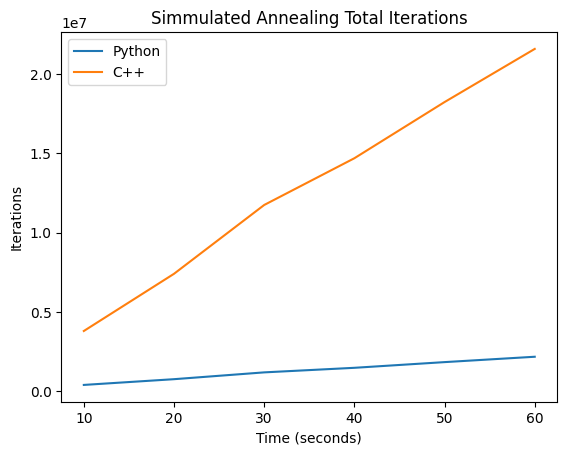
\includegraphics[scale=0.65]{images/TimeComparison.png}
\end{center}
As we see in the above comparison, the statically typed and compiled \texttt{C++} code significantly outperforms the number of iterations achieved by our Python program over equal run times by an order of 10. This results in our \texttt{C++} program being able to explore greater regions of the search space, and thus develop greater estimates of the global optimum assignment compared to our Python implementations. \\
\\
For particularly large instances of the QAP such as \texttt{tai256c}, this can result in a massive gap between the results of our experiments, and prior research \cite{1994Improved,Loiola07,stuzle,TATE199573}.


\newpage

\section{Conclusions}

All heuristics with the exception of our most basic Greedy constructive method proved to generate reasonable results within 60 seconds of compute time compared to the benchmark results of the QAP library. These results also imply the convergence of our methods to reasonable within our time limits. \\
\\
The success of our results can largely be attributed to borrowing proven techniques from prior research as discussed in section 2, as well as utilising sound software practices which we detail in our appendix. 



\subsubsection*{Future Work}
Whilst we implemented a number of heuristic approaches, we have only scratched the surface of methods explored within the extensive literature reviews \cite{article}. One immediate extension we could explore our work is further testing, and in particular extending the run time of our heuristics to the more common 1200 seconds CPU-Time standard which has been used in prior work \cite{stuzle, 1994Improved, TATE199573}. \\
\\
A more interesting extension however is to leverage parallelization as technique to enhance the performance. All algorithms considered in this report have been implemented \textit{sequentially}, that is, they are implemented by executing a sequence of operations over the input data. The idea of parallelization however is to user several independent processed to cooperated in order to compute a given task. The result is that if algorithm $A$ on input $n$ requires $Time_{A(n)}$ to compute, then a parallelizable implementation running on $p(n)$ processes can theoretically achieve this task in a much faster $Time_{A(n)}/p(n)$. Similar to our earlier remarks on the benefits of implementing our algorithms in a more computationally suitable language such as \texttt{C++}, the benefits of utilising parallelization is that the number of iterations achieved over the course of the algorithm can exceed that of the current sequential implementations; this in turn allows for greater exploration of the solution space within an equal time frame, allowing the algorithm to develop better solutions. \\
\\
Of course, parallelization is not a trivial task, nor a blunt instrument than can be applied to every heuristic; some algorithms are inherently sequential for example. However, exploring how these techniques can be used to enhance the performance of some of our implementations such as borrowing ideas from prior work on Genetic Algorithms and Parrellelization \cite{CANTUPAZ2000221}, as well as considering a parallelized \textit{multistart} approach to local search algorithms \cite{Gy_rgy_2011} could yield interesting results. For further references and inspiration on speedup by parallelization, we refer to chapter 7.5 of \cite{AlgorithmicsTextbook}. \\
\\
An additional aspect of our models that could be explored is their hyperparameters, particularly for Tabu Search, and Simulated Annealing. Given time and computational restrictions, we performed limited hyper-parameter tuning, to define fixed hyperparameters which we used across all instances we tested. Of course, this is sub-optimal, and different instances of the QAP could benefit from more specifically tuned hyperparameters. Future work and studies could explore sets of hyperparemeters for particular instances, or better yet, explore heuristics for constructing hyperparameters for a given instance of the QAP. \\
\\
Finally, we note that our work within this paper was relatively narrow; centering on the development of robust heuristics for the QAP, that would produce approximate results within the limited computational time of 60 CPU seconds. As has been well documented in \cite{AlgorithmicsTextbook}, the needs of practitioners may vary widely depending on their needs, and a focus on heuristic development for a 60 second CPU restriction may be far too narrow to be of interest to a wider audience. Future work could explore the convergence aspects of the heuristics developed within this paper, and instead focus on a convergence to CPU time ratio which may be of more interest to practioners.




\newpage
\section{Appendix of Implementation Details \& File Structure}
All methods discussed in section 2 are implemented in \texttt{Python} and conform to \href{https://en.wikipedia.org/wiki/Object-oriented_programming}{object orientated programming} (OOP) principals. All QAP heuristics are internally implemented as objects extending the following abstract base class: 
\begin{minted}{python}
    import numpy as np
    from time import time
    from abc import ABC, abstractmethod
    
    
    class QAP_heuristic(ABC):
        def __init__(self, w, d) -> None:
            assert w.shape == d.shape
            self.W = w
            self.D = d
            self.n = w.shape[0]
            self.MAX_CPU_TIME = time()+60  # sets 60s cap on runtime 
    
        @abstractmethod
        def solve(self, n_iter: int):
            pass
    
        def cost(self, X: np.array):
            return np.sum(self.W * self.D[X][:, X])       
\end{minted}
This abstract implementation requires each heuristic to implement the \texttt{solve} method, which encapsulates the essence of the heuristic. This allows us to abstract away common methods, such as computing the \textit{cost} function for a given assignment. For an example of how we leverage OOP, see the below implementation for iterated local search as per section 2 - with unnecessary details left obfuscated via \texttt{...}
\begin{minted}{python}
    class IteratedLocalSearch(QAP_heuristic):
        def __init__(self, w, d) -> None:
            super().__init__(w, d)
            self.n = w.shape[0]
        
        # Subroutines
        def generate_initial_solution(self):
            ...
        
        def local_search(self, perm: np.array):
            ...
        
        def acceptance_criterion(self, perm1: np.array, perm2: np.array):
            ...
        
        @staticmethod
        def peturbation(perm: np.array, k: int):
            ...
        
        # ILS implementation
        def solve(self, n_iters: int):
            s0 = self.generate_initial_solution()
            s  = self.local_search(s0)
            
            curr_best = s
            cost_history = [self.cost(s)]
            perm_history = [s]
    
            for _ in trange(n_iters):
                if time() > self.MAX_CPU_TIME: break  # breaks loop after 60s  
                s1 = self.peturbation(s, k=self.n//2)
                s2 = self.local_search(s1)
                curr_best = self.acceptance_criterion(curr_best, s2)
                
                cost_history.append(self.cost(curr_best))
                perm_history.append(curr_best)
    
            return curr_best
\end{minted}
By implementing heuristics this way, we are able to avoid needless anti-patterns as well as  bugs from redefining cost function calculations. This implementation also allows for efficient, automated testing of a heuristic by simply passing in an object instance. Moreover, by implementing our heuristics this way, we allow for a more equitable comparison between each method; as they differ in only how the \texttt{solve} procedure operates. \\
\\
In addition to streamlining the implementation of our heuristics, we also 
developed a class for testing QAP heuristics which automates our testing suite for ease of research. The aptly titled \texttt{QAP\_Tester} class implements the following method for testing a given heuristic

\begin{minted}{python}
    def test_hueristic(self, n_iters: int, n_trials: int, 
                       tai_only=False, bur_only=False, **kwargs):
        """
        tests the hueristic over specified number of trials and iterations. 
        records avg gap, std. dev, max gap, min gap for each trial
        """
        results_filename = self.write_to_path + str(self.heuristic)

        if tai_only: results_filename += '-tai.csv'
        if bur_only: results_filename += '-bur.csv'
        if not tai_only and not bur_only: filename += '.csvs'

        # we open with append mode, to avoid wiping an entire DB of results
        with open(results_filename, mode='a') as results:  
            
            writer = csv.writer(results)
            writer.writerow(['instance', 'avg gap', 'std_dev', 
                             'max gap', 'min gap', 'trials'])


            for filename in os.listdir(self.instance_path): 
                
                 # skips any instances that are not Tai
                if tai_only and 'tai' not in filename: continue    
                if bur_only and 'bur' not in filename: continue

                file_it = iter(self.__read_integers(self.instance_path+filename))

                # open QAP instance param's 
                n = next(file_it)
                w = np.array([[next(file_it) for j in range(n)] for i in range(n)])
                d = np.array([[next(file_it) for j in range(n)] for i in range(n)])

                soln_file = filename[:-4]+'.sln' # this removes the .dat from filename

                try:
                    
                    gaps = []
                    qap_soln = self.__open_solution(self.soln_path+soln_file)

                    for _ in range(n_trials): 
                        # create an instance and run test
                        heuristic = self.heuristic(w,d,**kwargs)
                        huerstic_soln = heuristic.solve(n_iters)
                        gap = 100*(heuristic.cost(huerstic_soln) - qap_soln)/qap_soln
                        gaps.append(gap)

                    writer.writerow([filename, np.mean(gaps), np.std(gaps), 
                                     max(gaps), min(gaps), n_trials])
                
            # any instances without corresponding solution files are deleted
                except FileNotFoundError:
                    os.remove(self.instance_path+filename)        
        return
\end{minted}

\subsubsection*{File Structure \& Replication of Results}
For a thorough description of our file structure we refer to the \texttt{README} section of our now public \href{https://github.com/Seannnnnnnnnnn/QAP}{\texttt{GitHub} repository}. Within each of the associated \texttt{.ipynb} files for our heuristics details in section 2, results can be reproduced by running all cells, and then executing the \texttt{Tester.test\_heuristic} specified earlier in the appendix. \\
\\
We do note however that all results were generated in our experimental environment as detailed in section 3, and results may very depending on the hardware on which our implementations are tested.



\newpage
\bibliographystyle{unsrt}%Used BibTeX style is unsrt
\bibliography{sample}


\end{document}
